%-*-latex-*-
\sectionthree{Distribution sort: counting sort}
\begin{python0}
from solutions import *; clear()
\end{python0}

Beside sorting an array using a comparison-based sorting
algorithm, i.e., using $\leq$ or $<$ or $\geq$ or $>$ to compare values in the array,
there's
another class of sorting algorithms that work in a difference way.
Distribution sorting algoroithms sort by \textit{distributing}
the values in an array.
Sometimes distribution sort will use a comparison-based sort.

The simplest distribution sort is the counting sort.

Suppose you have an array \verb!x! of integers with values
from 0 to 4 (inclusive):


\begin{center}
\begin{tikzpicture}[>=triangle 60,shorten >=0.5pt,node distance=2cm,auto,initial text=, double distance=2pt]
\node[state] (A) at (  3,  0) {$A$};
\node[state] (B) at (  6,  0) {$B$};
\node[state] (S) at (  0, -2) {$S$};
\node[state] (C) at (  3, -4) {$C$};

\path[->]
(A) edge [bend left=0,pos=0.5,above] node {} (B)
(A) edge [bend left=0,pos=0.5] node {} (C)
(S) edge [bend left=0,pos=0.5,above] node {} (A)
(S) edge [bend left=0,pos=0.5,above] node {} (C)

;
\end{tikzpicture}
\end{center}
    


You scan the array and count the number of times each value
from 0 to 4 occurs in \verb!x!.

%-*-latex-*-
{\footnotesize \begin{Verbatim}[frame=single,fontsize=\small]
[student@localhost discrete-probability] python tossfaircoin2.py
experiment 0 ... outcome: TAIL
experiment 1 ... outcome: TAIL
experiment 2 ... outcome: TAIL
experiment 3 ... outcome: TAIL
experiment 4 ... outcome: TAIL
experiment 5 ... outcome: TAIL
experiment 6 ... outcome: HEAD
experiment 7 ... outcome: TAIL
experiment 8 ... outcome: TAIL
experiment 9 ... outcome: TAIL
experiment 10 ... outcome: TAIL
experiment 11 ... outcome: HEAD
experiment 12 ... outcome: HEAD
experiment 13 ... outcome: TAIL
experiment 14 ... outcome: HEAD
experiment 15 ... outcome: TAIL
experiment 16 ... outcome: TAIL
experiment 17 ... outcome: HEAD
experiment 18 ... outcome: HEAD
experiment 19 ... outcome: TAIL
number of experiments: 20
number of heads: 6
number of tails: 14
probability of getting head: 0.3
probability of getting tail: 0.7
\end{Verbatim}
}


For instance \verb!count[2]! is the number of times \verb!2!
occurs in array \verb!x!.

Now the final thing to do is to fill \verb!x! using
information in \verb!count!.
For instance \verb!count[0]! is \verb!2!, 
so I would put two \verb!0!'s into \verb!x!:

\begin{console}
12094
\end{console}


Next, since \verb!count[1]! is \verb!0!, \verb!1! does not appear in 
\verb!x!.
So the re-organized \verb!x! looks like this (i.e., no change):

\begin{center}
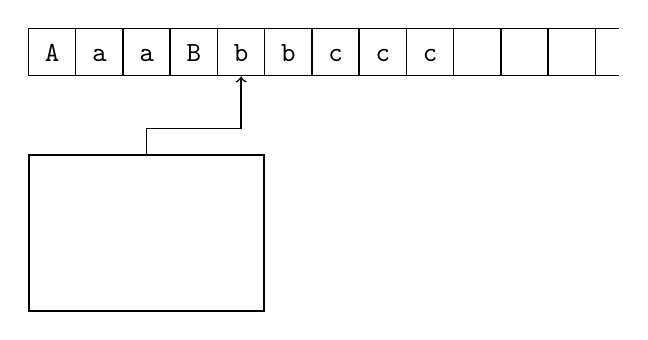
\begin{tikzpicture}

\draw (0.3, 0.3)
  node[draw, line width=0.02cm, , color=black,
       rounded corners=0cm, inner sep=0cm] {

\begin{minipage}[t][0.6cm]{0.6cm}
\mbox{}

\end{minipage}

};\draw (0.3, 0.3) node[color=black] {{\vphantom{AaaBbbccc$\BLANK$$\BLANK$$\BLANK$}\texttt{A}}};
\draw (0.8999999999999999, 0.3)
  node[draw, line width=0.02cm, , color=black,
       rounded corners=0cm, inner sep=0cm] {

\begin{minipage}[t][0.6cm]{0.6cm}
\mbox{}

\end{minipage}

};\draw (0.8999999999999999, 0.3) node[color=black] {{\vphantom{AaaBbbccc$\BLANK$$\BLANK$$\BLANK$}\texttt{a}}};
\draw (1.5, 0.3)
  node[draw, line width=0.02cm, , color=black,
       rounded corners=0cm, inner sep=0cm] {

\begin{minipage}[t][0.6cm]{0.6cm}
\mbox{}

\end{minipage}

};\draw (1.5, 0.3) node[color=black] {{\vphantom{AaaBbbccc$\BLANK$$\BLANK$$\BLANK$}\texttt{a}}};
\draw (2.0999999999999996, 0.3)
  node[draw, line width=0.02cm, , color=black,
       rounded corners=0cm, inner sep=0cm] {

\begin{minipage}[t][0.6cm]{0.6cm}
\mbox{}

\end{minipage}

};\draw (2.0999999999999996, 0.3) node[color=black] {{\vphantom{AaaBbbccc$\BLANK$$\BLANK$$\BLANK$}\texttt{B}}};
\draw (2.7, 0.3)
  node[draw, line width=0.02cm, , color=black,
       rounded corners=0cm, inner sep=0cm] {

\begin{minipage}[t][0.6cm]{0.6cm}
\mbox{}

\end{minipage}

};\draw (2.7, 0.3) node[color=black] {{\vphantom{AaaBbbccc$\BLANK$$\BLANK$$\BLANK$}\texttt{b}}};
\draw (3.3, 0.3)
  node[draw, line width=0.02cm, , color=black,
       rounded corners=0cm, inner sep=0cm] {

\begin{minipage}[t][0.6cm]{0.6cm}
\mbox{}

\end{minipage}

};\draw (3.3, 0.3) node[color=black] {{\vphantom{AaaBbbccc$\BLANK$$\BLANK$$\BLANK$}\texttt{b}}};
\draw (3.9000000000000004, 0.3)
  node[draw, line width=0.02cm, , color=black,
       rounded corners=0cm, inner sep=0cm] {

\begin{minipage}[t][0.6cm]{0.6cm}
\mbox{}

\end{minipage}

};\draw (3.9000000000000004, 0.3) node[color=black] {{\vphantom{AaaBbbccc$\BLANK$$\BLANK$$\BLANK$}\texttt{c}}};
\draw (4.5, 0.3)
  node[draw, line width=0.02cm, , color=black,
       rounded corners=0cm, inner sep=0cm] {

\begin{minipage}[t][0.6cm]{0.6cm}
\mbox{}

\end{minipage}

};\draw (4.5, 0.3) node[color=black] {{\vphantom{AaaBbbccc$\BLANK$$\BLANK$$\BLANK$}\texttt{c}}};
\draw (5.1, 0.3)
  node[draw, line width=0.02cm, , color=black,
       rounded corners=0cm, inner sep=0cm] {

\begin{minipage}[t][0.6cm]{0.6cm}
\mbox{}

\end{minipage}

};\draw (5.1, 0.3) node[color=black] {{\vphantom{AaaBbbccc$\BLANK$$\BLANK$$\BLANK$}\texttt{c}}};
\draw (5.699999999999999, 0.3)
  node[draw, line width=0.02cm, , color=black,
       rounded corners=0cm, inner sep=0cm] {

\begin{minipage}[t][0.6cm]{0.6cm}
\mbox{}

\end{minipage}

};\draw (5.699999999999999, 0.3) node[color=black] {{\vphantom{AaaBbbccc$\BLANK$$\BLANK$$\BLANK$}\texttt{$\BLANK$}}};
\draw (6.299999999999999, 0.3)
  node[draw, line width=0.02cm, , color=black,
       rounded corners=0cm, inner sep=0cm] {

\begin{minipage}[t][0.6cm]{0.6cm}
\mbox{}

\end{minipage}

};\draw (6.299999999999999, 0.3) node[color=black] {{\vphantom{AaaBbbccc$\BLANK$$\BLANK$$\BLANK$}\texttt{$\BLANK$}}};
\draw (6.899999999999999, 0.3)
  node[draw, line width=0.02cm, , color=black,
       rounded corners=0cm, inner sep=0cm] {

\begin{minipage}[t][0.6cm]{0.6cm}
\mbox{}

\end{minipage}

};\draw (6.899999999999999, 0.3) node[color=black] {{\vphantom{AaaBbbccc$\BLANK$$\BLANK$$\BLANK$}\texttt{$\BLANK$}}};\draw[line width=0.02cm,black] (7.1999999999999975,0.6) to  (7.499999999999998,0.6);
\draw[line width=0.02cm,black] (7.1999999999999975,0.0) to  (7.499999999999998,0.0);

\draw (1.5, -2.0)
  node[draw, line width=0.02cm, , color=black,
       rounded corners=0cm, inner sep=0cm] {

\begin{minipage}[t][1.98cm]{2.98cm}
\mbox{}

\end{minipage}

};\draw[line width=0.02cm,black,->] (1.5,-1) to  (1.5,-0.67) to  (2.7,-0.67) to  (2.7,-0.01);
\end{tikzpicture}

\end{center}



However note that \verb!count[2]! is \verb!3!, which means that
\verb!2! appears \verb!3! times.
Therefore my \verb!x! now look like this:

%-*-latex-*-
\begin{Verbatim}[frame=single,fontsize=\small]
[student@localhost discrete-probability] python discrete-probrobability/game2.py
python: can't open file 'discrete-probrobability/game2.py': [Errno 2] No such fi
le or directory
\end{Verbatim}



You get the point.

The pseudocode looks like this.
I assume that the values in \verb!x! are from 0 to \verb!M!.
\begin{console}
ALGORITHM: counting_sort
INPUT: array x of size n

    count = int array of size M + 1, initialized with 0s
    for i = 0, 1, 2, ..., n - 1:
        count[x[i]] = count[x[i]] + 1
    j = 0
    for i = 0, 1, 2, ..., M:
        for k = 1, ..., count[i]:
            x[j] = i
            j = j + 1
\end{console}

If \verb!M! is not 
known, you have to run through \verb!x! to figure that out.


Here's the runtime analysis.
The time to create \verb!count!, if it's in the heap,
might very well be $O(1)$ (or the memory allocation might fail because of lack of
available memory). So that's hard to say.
So let's just assume memory allocation for \verb!count! is negligible.
First you have to set the \verb!count! array to zeroes:
that takes $A(M + 1)$ ($A$ is a constant).
You need to run through \verb!x! to fill \verb!count! with
values: that takes a time of $Bn$.
You will to put values back into \verb!x! using \verb!count!.
That requires touching each cell in \verb!x!.
So for this part, the runtime is $Cn$.
Altogether, the runtime is
\[
O(n + M)
\]
Of course the space requirement is
\[
O(M + 1) = O(M)
\]


\begin{ex} 
  \label{ex:some-decision1}
  \tinysidebar{\debug{exercises/{empty0/question.tex}}}
  \solutionlink{sol:some-decision1}
  \qed
\end{ex} 
\begin{python0}
from solutions import *
add(label="ex:some-decision1",
    srcfilename='exercises/some-decision1/answer.tex') 
\end{python0}



\begin{ex} 
  \label{ex:some-decision1}
  \tinysidebar{\debug{exercises/{empty0/question.tex}}}
  \solutionlink{sol:some-decision1}
  \qed
\end{ex} 
\begin{python0}
from solutions import *
add(label="ex:some-decision1",
    srcfilename='exercises/some-decision1/answer.tex') 
\end{python0}



\begin{ex} 
  \label{ex:some-decision1}
  \tinysidebar{\debug{exercises/{empty0/question.tex}}}
  \solutionlink{sol:some-decision1}
  \qed
\end{ex} 
\begin{python0}
from solutions import *
add(label="ex:some-decision1",
    srcfilename='exercises/some-decision1/answer.tex') 
\end{python0}



\begin{ex} 
  \label{ex:some-decision1}
  \tinysidebar{\debug{exercises/{empty0/question.tex}}}
  \solutionlink{sol:some-decision1}
  \qed
\end{ex} 
\begin{python0}
from solutions import *
add(label="ex:some-decision1",
    srcfilename='exercises/some-decision1/answer.tex') 
\end{python0}

